\documentclass[10pt, t]{beamer}
\usetheme{metropolis}           % Use metropolis theme

\usepackage{appendixnumberbeamer}

\ifnotes
  \hypersetup{final}
  \usepackage{pgfpages}
  \setbeamertemplate{note page}[plain]
  \setbeameroption{show notes on second screen=right}
\fi

\usepackage{verbatim}

\usepackage{listings}

\usepackage[scale=3]{ccicons}   % creative commons icons

\title{Introduction to parallel computing}
\date{}
\author{Jeremy Iverson}
\institute{College of Saint Benedict \& Saint John's University}
\begin{document}
  \maketitle

  \begin{frame}{cpu performance}
    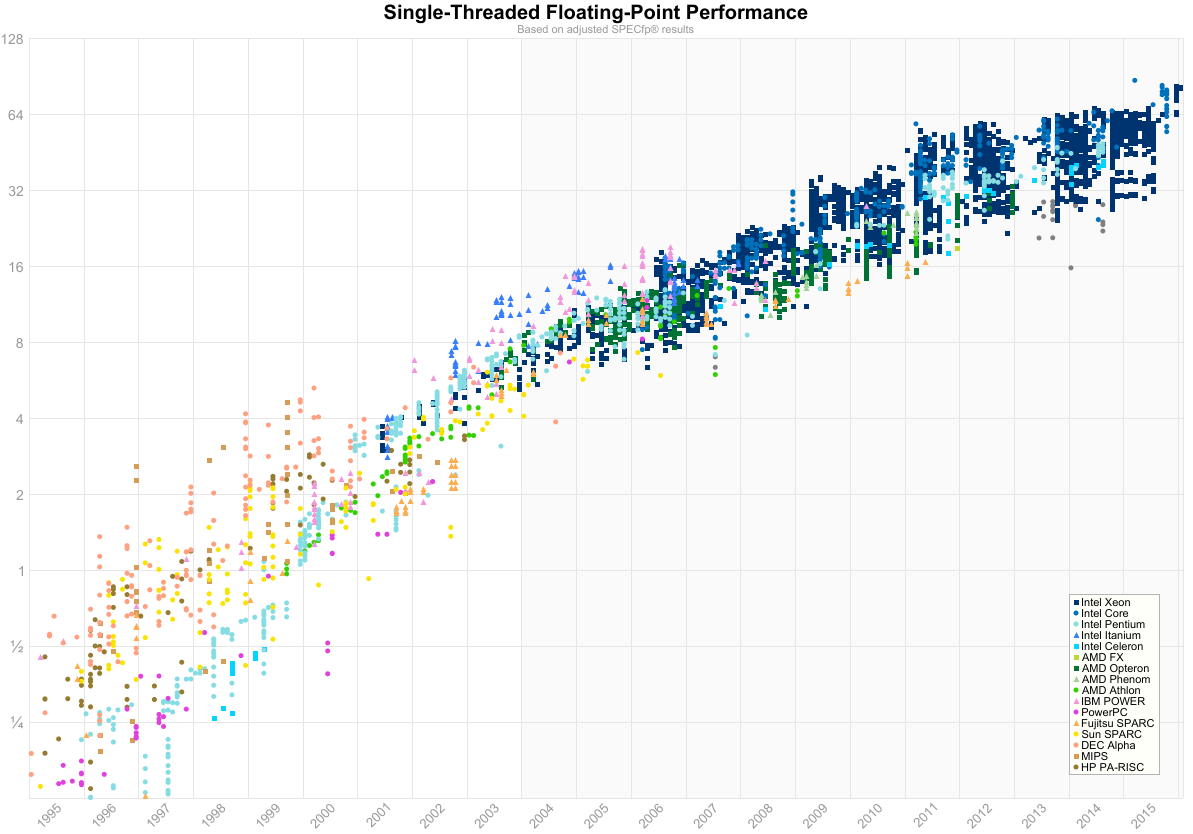
\includegraphics[width=\textwidth]{float-point-perf.png}\\
    \hfill \tiny{\href{http://imgur.com/a/2fiLF}{Single-Threaded~Floating-point~Performance}~by~HenkPoley}
    \note{\begin{itemize}
      \item the ``almost'' current state of things
      \item what do you notice about this graph?
        \begin{itemize}
          \item from 1986 -- 2002, microprocessor performance increased by
            roughly 50\% every two years, since then it has dropped to about
            20\%
        \end{itemize}
    \end{itemize}}
  \end{frame}

  \begin{frame}{clock speed}
    \vspace{2.5ex}
    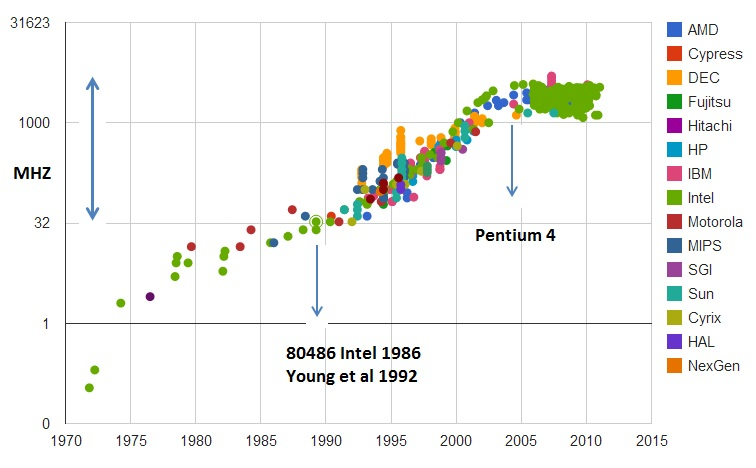
\includegraphics[width=\textwidth]{Clock_CPU_Scaling.jpg}\\
    \hfill
    \tiny{\href{https://en.wikipedia.org/wiki/File:Clock_CPU_Scaling.jpg}{Clock~CPU~Scaling.jpg}~by~Newhorizons~msk~/~\href{http://creativecommons.org/publicdomain/zero/1.0}{CC0~1.0}}

    \note{
      \begin{itemize}
        \item do you notice anything odd about this graph, given the previous
          graph?
          \begin{itemize}
            \item we are seeing \textasciitilde20\% performance improvement
              despite stagnating clock speed
          \end{itemize}
        \item why does clock speed stop increasing?
          \begin{itemize}
            \item faster processor = increased power consumption.
            \item increased power consumption = increased heat.
            \item increased heat = unreliable processors.
          \end{itemize}
        \item we are reaching / have reached the limit that current cooling
          technologies can remove heat from the chip (a.k.a. the power wall)
        \item so how does performance improve, when clock speed plateaus?
      \end{itemize}
    }
  \end{frame}

  \begin{frame}{transistor count}
    \vspace{1.5ex}
    \centering
    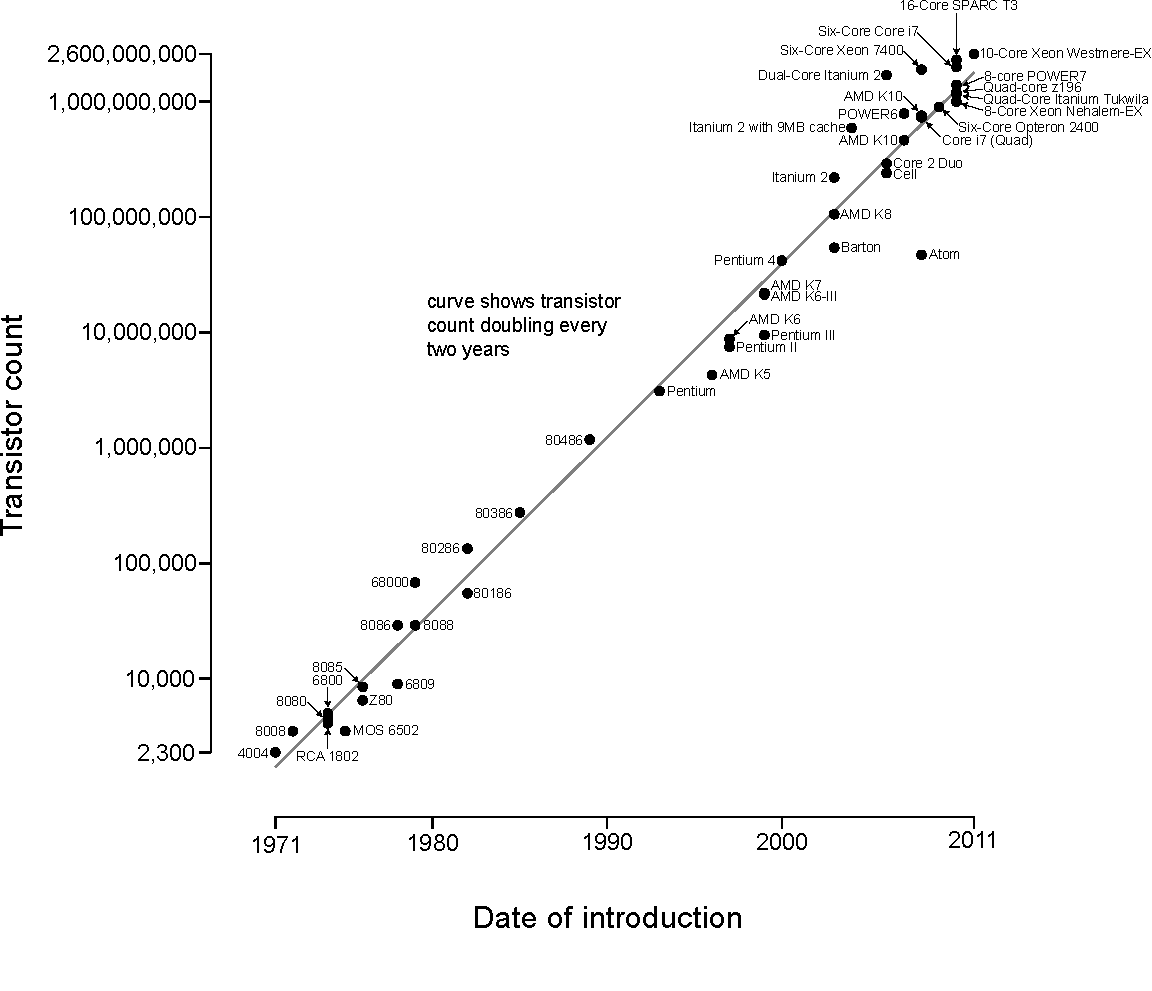
\includegraphics[width=.75\textwidth]{Transistor_Count_and_Moore's_Law_-_2011.pdf}\\
    \hfill \tiny{\href{https://en.wikipedia.org/wiki/Moore's\_law\#/media/File:Transistor\_Count\_and\_Moore's\_Law\_-\_2011.svg}{Transistor~Count~and~Moore's~Law~-~2011}~by~Wgsimon~/~\href{http://creativecommons.org/licenses/by-sa/3.0}{CC~BY~3.0}~/~cropped~from~original}

    \note{
      \begin{itemize}
        \item pre 2005 --- a golden era when clock speed could be increased
          while adding more transistors, which resulted in the large performance
          improvements in the first graph
        \item post 2005 --- performance improvements now have to come from more
          advanced chip capabilities
        \item we don't speed up the processor, we make it more sophisticated
          \begin{itemize}
            \item larger data busses
            \item larger caches
            \item deeper instruction pipelines (ILP)
          \end{itemize}
        \item Moore's law (c. 1965) --- transistor count roughly doubles every
          two years
        \item so, how can we keep continue to improve performance?
      \end{itemize}
    }
  \end{frame}

  \begin{frame}{supercomputer performance}
    \centering
    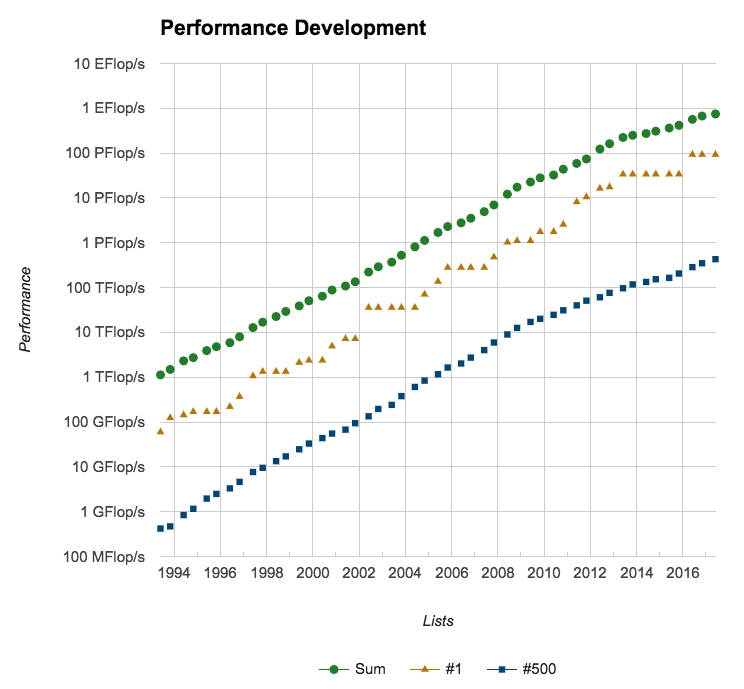
\includegraphics[width=.7\textwidth]{top500.png}\\
    \hfill \tiny{Graph courtesy of \href{https://www.top500.org/statistics/perfdevel/}{The Top 500 List.}\hspace{.15\textwidth}}

    \note{
      \begin{itemize}
        \item so how does any of this affect us, in this class?
        \item notice anything about this graph?
          \begin{itemize}
            \item performance improvement is exponential
            \item how can that be?
              \begin{itemize}
                \item we are no longer constrained by the limitations of a
                  single chip
                \item so what are our limitations?
              \end{itemize}
          \end{itemize}
      \end{itemize}
    }
  \end{frame}

  \begin{frame}[standout]
    what are the challenges of parallel computing?

    \note{
      \begin{itemize}
        \item how do we take advantage of available parallel resources, i.e.,
          how to convert serial programs to parallel programs
          \begin{itemize}
            \item automatic translation has been attempted and is still being
              studied, but success has been limited
          \end{itemize}
      \end{itemize}
    }
  \end{frame}

  \newsavebox{\LstA}
  \begin{lrbox}{\LstA}
    \begin{lstlisting}
      for (int i=0; i<n; ++i) {
        a[0] += a[i];
      }
    \end{lstlisting}
  \end{lrbox}

  \begin{frame}[fragile]{counting}
    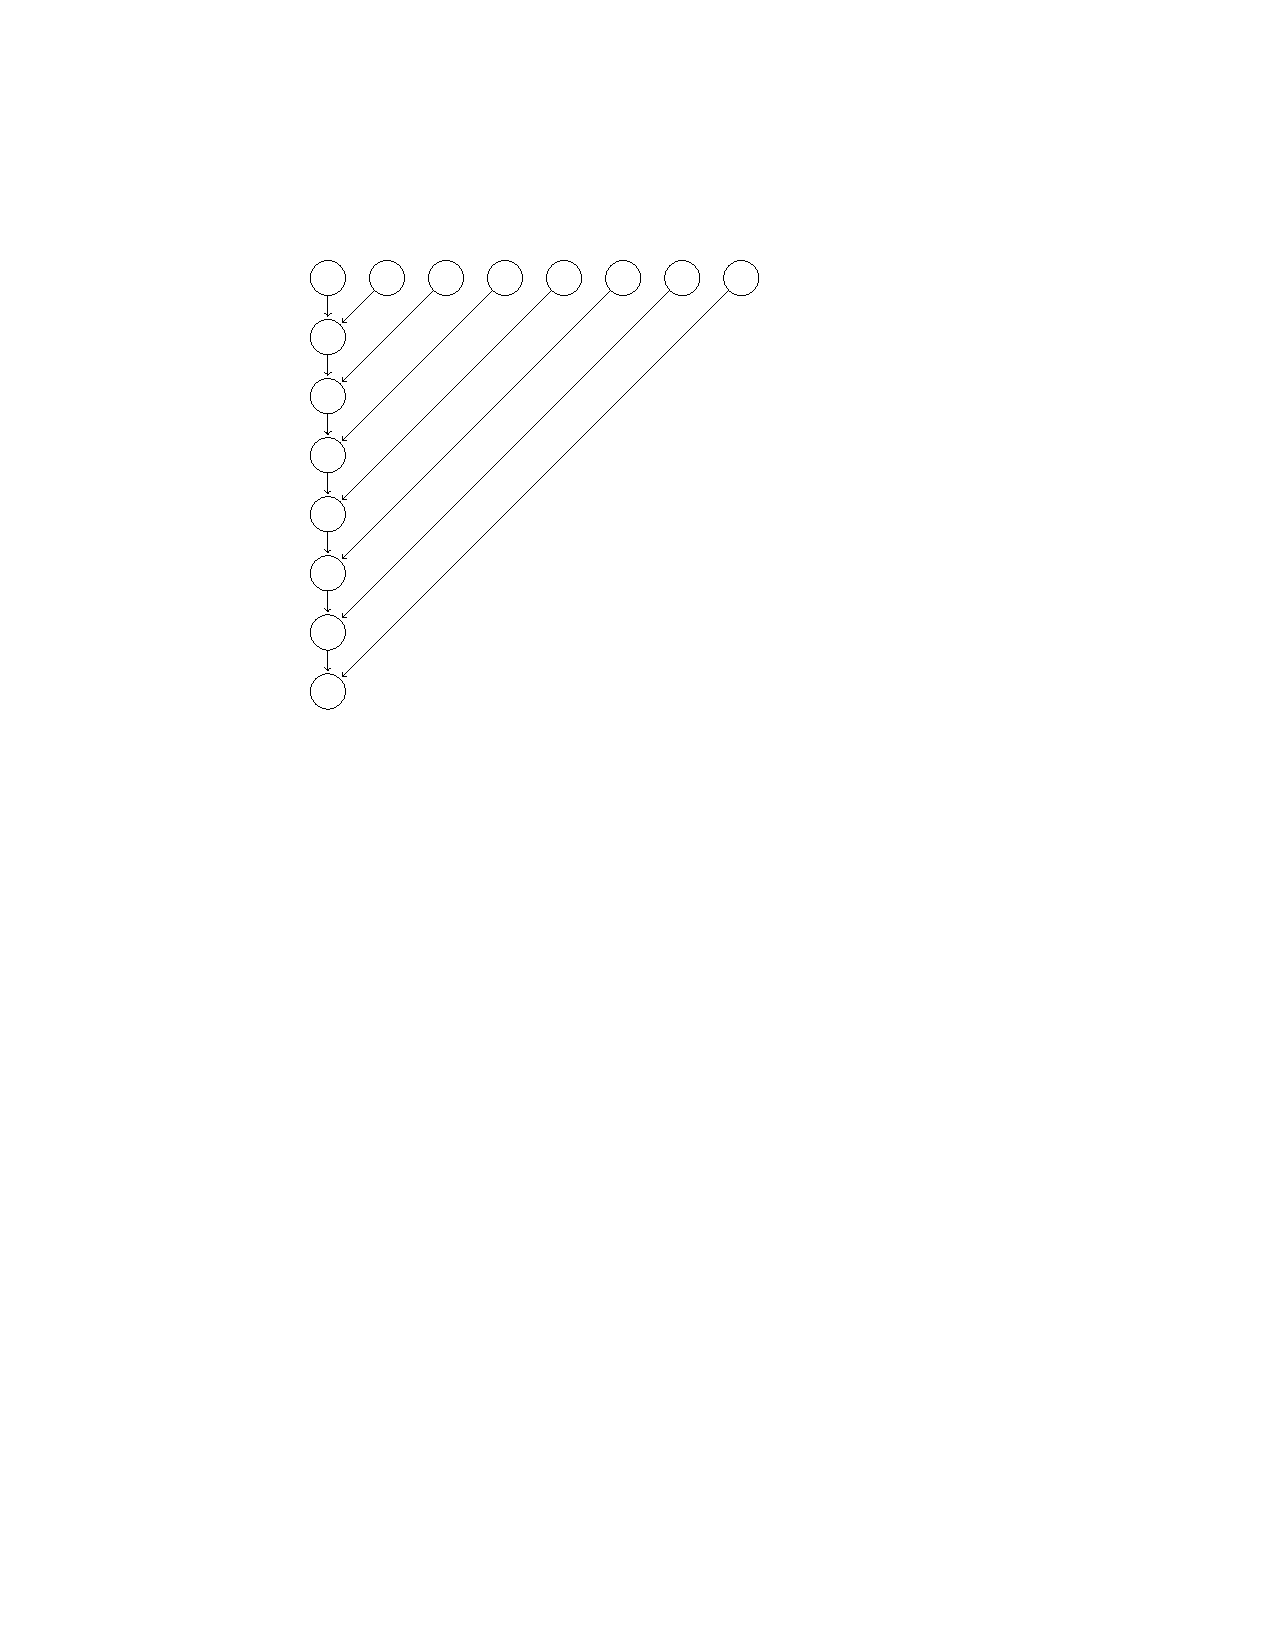
\includegraphics[width=\textwidth]{serial.pdf}

    \note{
      \begin{itemize}
        \item how many steps, described as a function of the number of nodes?
        \item where are there dependencies / why can't this be parallelized?
      \end{itemize}

      \par\usebox{\LstA}
    }
  \end{frame}

  \begin{frame}{counting cont.}
    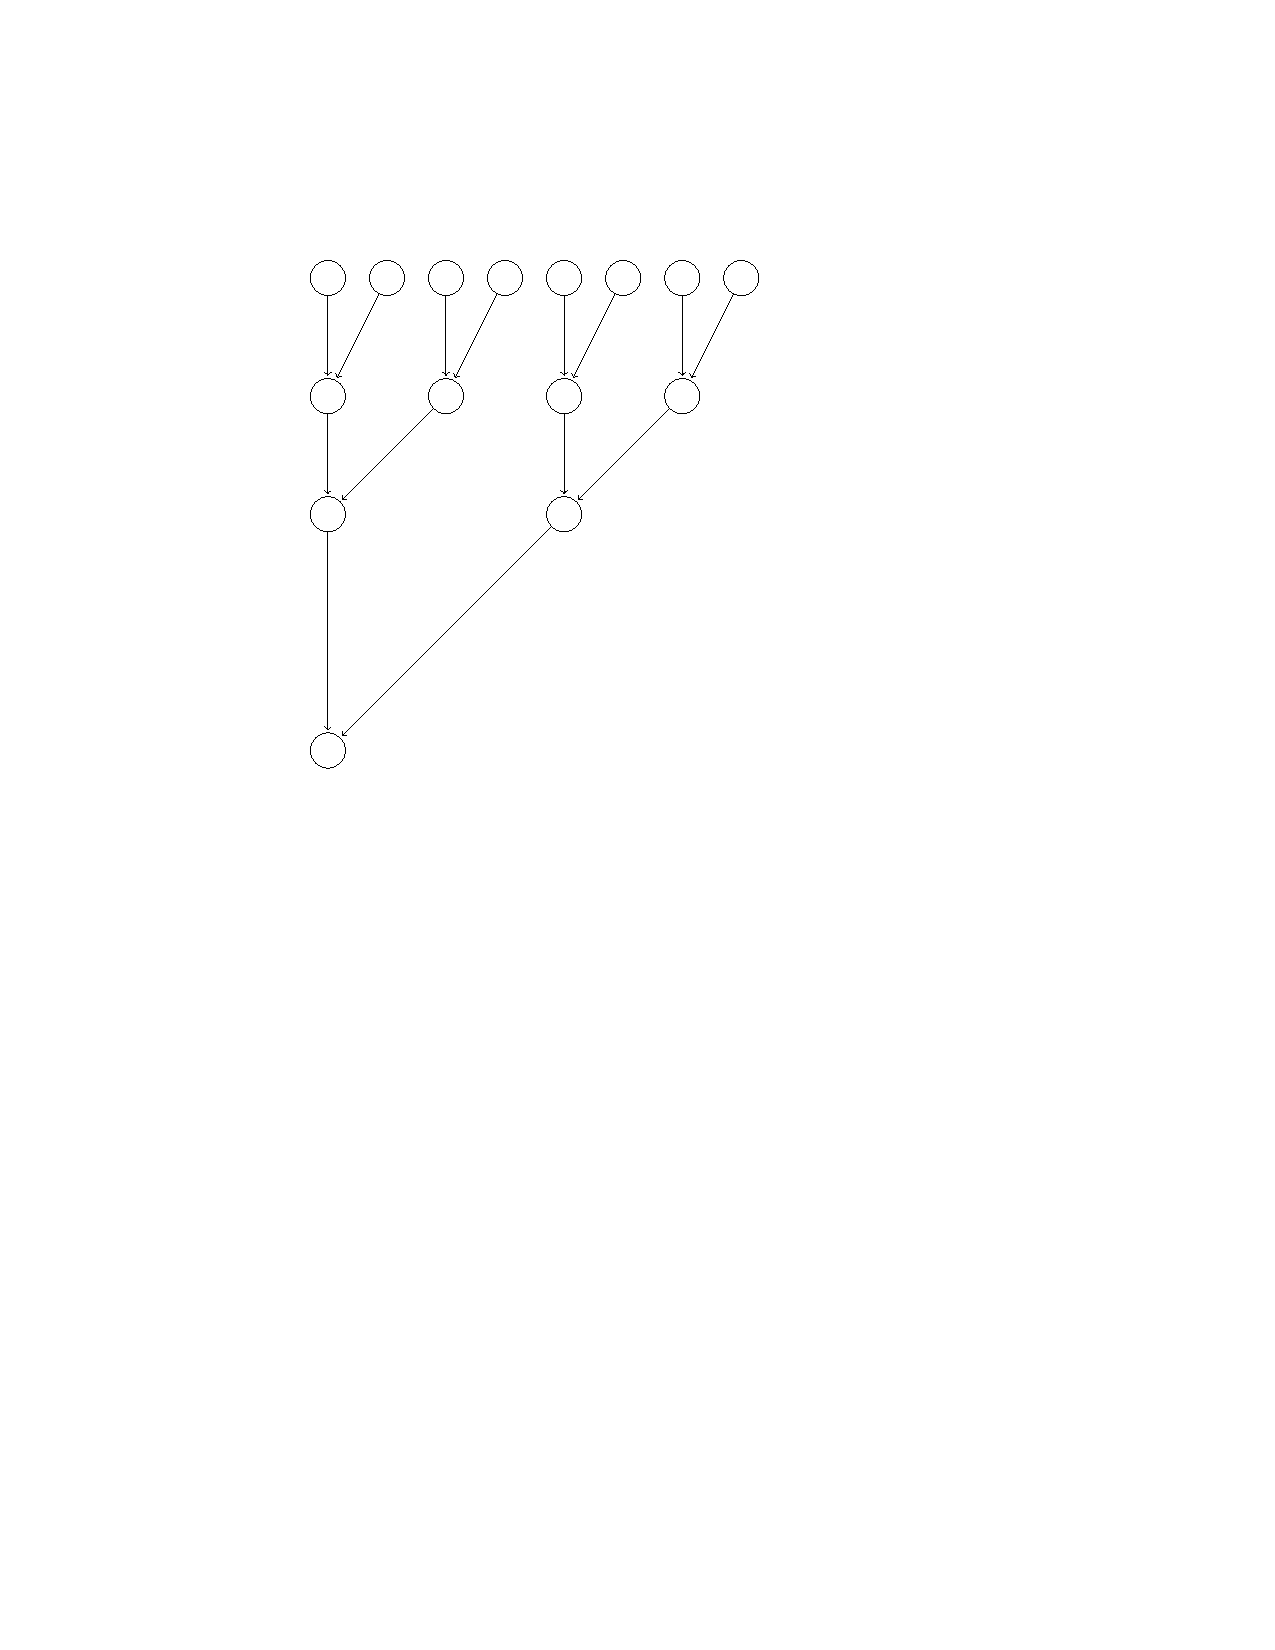
\includegraphics[width=\textwidth]{parallel.pdf}

    \note{
      \begin{itemize}
        \item how many steps, described as a function of the number of nodes?
        \item what happens if the number of nodes is not a power of two?
        \item what would the code look like to accomplish this (what do you need
          to express, that you do not know how)?
      \end{itemize}
    }
  \end{frame}

  \appendix

  \begin{frame}[c]
    \begin{center}\ccbysa\end{center}

    except where otherwise noted, this worked is licensed under
    \href{http://creativecommons.org/licenses/by-sa/4.0/}{creative commons
    attribution-sharealike 4.0 international license}
  \end{frame}
\end{document}
